\pdfinfo{
    /Author (Ippolito Lavorati, Andrea Bruttomesso)
    /Title (Travelling Salesman Problem (TSP))
    /Keyword (TSP, Heuristic, CPLEX)
}

% Libraries
\documentclass[a4paper,12pt]{report}
\usepackage[utf8]{inputenc}
\usepackage[english]{babel}
\usepackage{fancyhdr}
\usepackage{sectsty}
\usepackage[inner=3cm,top=2cm,bottom=2cm,outer=2cm]{geometry}
\usepackage{setspace}
\usepackage[hang,small,sf,font=small, labelfont=bf]{caption}
\usepackage{subcaption}
\usepackage[usenames]{color}
\usepackage{xcolor}
\usepackage{colortbl}
\usepackage{tocloft}
\usepackage[a-1b]{pdfx}
\usepackage{hyperref}
\usepackage{tabto}
\usepackage{mathtools}
\usepackage{bbold}
\usepackage{wrapfig}
\usepackage[]{mdframed}
\usepackage{amsmath}
\usepackage{amsthm}
\usepackage{amssymb}
\usepackage{cases}
\usepackage{indentfirst}
\usepackage{afterpage}
\usepackage{placeins}
\usepackage{csquotes}
\usepackage{abstract}
\usepackage{todonotes}

%images
\usepackage{graphicx}
\graphicspath{ {./images/} }

%tikz
\usepackage{tikz}
\usetikzlibrary{arrows.meta}

%pseudocode
\usepackage{algorithm}
\usepackage{algpseudocode}

\DeclarePairedDelimiter\floor{\lfloor}{\rfloor}
\DeclarePairedDelimiter\ceil{\lceil}{\rceil}
\setlength{\arrayrulewidth}{1pt}
\newcommand\blankpage{%
    \null
    \thispagestyle{empty}%
    \addtocounter{page}{-1}%
    \newpage}

% Mandatory settings
\onehalfspacing
\hypersetup{
    colorlinks,
    citecolor=black,
    filecolor=black,
    linkcolor=black,
    urlcolor=black
}

% Subsections
\renewcommand{\cftpartleader}{\cftdotfill{\cftdotsep}} % for parts
\renewcommand{\cftchapleader}{\cftdotfill{\cftdotsep}} % for chapters
\renewcommand{\cftsecleader}{\cftdotfill{\cftdotsep}} % for sections
\renewcommand{\listfigurename}{List of performance profiles}

\algnewcommand\algorithmicforeach{\textbf{for each}}
\algdef{S}[FOR]{ForEach}[1]{\algorithmicforeach\ #1\ \algorithmicdo}


\usepackage[sorting=none]{biblatex}

\addbibresource{bibl.bib}





% Start document
\begin{document}

\begin{titlepage}
\begin{center}


\includegraphics[height=0.13\textheight]{logo_unipd.png}
\hfill

\includegraphics[height=0.13\textheight]{logo_dei.png}
\newline
\newline

\vspace{0.8cm}
\textsc{\LARGE Universit\`{a} degli Studi di Padova}\\
\vspace{1.6cm}
\textsc{\large 	School of Engineering Department of Information Engineering}\\
\vspace{0.4cm}

\textsc{\large Master Degree in Computer Engineering}\\
\vfill
{ \LARGE \bfseries Performance analysis on Traveling Salesman Problem solving techniques}\\
\vspace{.2cm}

\textbf{\large Operations Research 2}\\
\vfill

\raggedright\textbf{\large Supervisor:} \\
\raggedright\large Matteo Fischetti\\
\vfill
\raggedright\textbf{\large Candidates:} \\
\raggedright\large Ippolito Lavorati  (2131127)\\
\raggedright\large Andrea Bruttomesso (2120933)\\

\vfill
\centering{Academic Year 2024/2025}

\end{center}
\end{titlepage}

%\pagenumbering{roman}
%\thispagestyle{empty}
%\clearpage{\pagestyle{plain}\cleardoublepage}
    
%\clearpage\null\newpage

% Abstract
%\newcommand\summaryname{Abstract}
%\newenvironment{Abstract} {
%    \begin{center}%
%    \bfseries{\summaryname} \end{center}
%}
    
\begin{abstract}
The Travelling Salesman Problem (TSP) is a fundamental and widely studied optimization problem in the field of Operations Research. It consists of finding the shortest possible route that visits a set of cities exactly once and returns to the starting point. Despite its simple formulation, the TSP is NP-hard, making it computationally challenging to solve for large instances.

Over the decades, a variety of algorithmic approaches have been developed to tackle the problem, ranging from exact methods to heuristics and metaheuristics. Among these, Concorde represents the state-of-the-art in exact TSP solvers, leveraging advanced optimization techniques. However, such high-performance tools are often complex and computationally demanding.

This thesis aims to explore and compare a selection of more accessible algorithmic strategies, including classical heuristics and metaheuristics. Through implementation and experimental evaluation, the work provides insights into their practical performance and highlights the trade-offs between computational efficiency and solution quality in solving the TSP.

\end{abstract}

% Index
\clearpage{\pagestyle{plain}\cleardoublepage}
\tableofcontents
%\listoftables

\clearpage{\pagestyle{plain}\cleardoublepage}
\pagenumbering{arabic}

%\afterpage{\blankpage}

% Introduction
\clearpage{\pagestyle{plain}\cleardoublepage}
\chapter{Introduction}
Travel \cite{Glover1990}
\chapter{Heuristic}
A heuristic is a practical problem-solving technique designed to produce good-enough solutions within a reasonable time frame, 
especially when exact methods are too slow or infeasible. Given the NP-hard nature of the Travelling Salesman Problem (TSP), 
computing the optimal solution can be computationally expensive even for moderately sized instances. For this reason, heuristic methods 
play a crucial role in tackling the problem efficiently. Heuristics do not guarantee optimality, but they can often yield solutions 
that are sufficiently close to the best possible one. This trade-off between accuracy and speed makes heuristics particularly valuable 
when timely decision-making is more important than absolute precision.

In this chapter, several heuristic strategies for the TSP are presented, highlighting their underlying principles, implementation, and performance.

\section{Nearest Neighbour - Greedy}

One of the most intuitive heuristic approaches to the Travelling Salesman Problem is the \textbf{Nearest Neighbor} (NN) algorithm, which follows a greedy strategy. 
A \textit{greedy} algorithm builds a solution step by step by always choosing the locally optimal option, with the hope that this leads to a good global solution.
In the context of the TSP, the algorithm starts from an initial node and, at each iteration, selects the nearest unvisited node as the next step in the tour. 
This process continues until all nodes have been visited exactly once, and the cycle is closed by returning to the starting point.
However, the quality of the solution obtained using this method depends heavily on the starting node, as different starting points may lead to significantly 
different tours.
While NN is fast and easy to implement, its performance depends heavily on the starting node and often produces suboptimal solutions. Still, it often produces a reasonable approximation in a fraction of the time required by exact methods, making it suitable for large instances where exact algorithms are computationally expensive.

\begin{algorithm}
\caption{Nearest Neighbor Heuristic}
\begin{algorithmic}
  \Require Starting node $s \in V$
  \Ensure Hamiltonian cycle of $G$, cost of cycle
  \State $cycle \gets [s]$
  \State $cost \gets 0$
  \For{$i \gets 0$ to $|V| - 2$}
    \State $next \gets \arg\min_{v \in V \setminus cycle} c(cycle[i], v)$
    \State $cost \gets cost + c(cycle[i], next)$
    \State $cycle[i+1] \gets next$
  \EndFor
  \State $cost \gets cost + c(cycle[|V| - 1], s)$
  \State \Return $cycle$, $cost$
\end{algorithmic}
\end{algorithm}

\subsection{Results Analysis}
\label{sec:nn-analysis}
The greedy algorithm often selects locally optimal edges without considering long-term implications, which may lead to expensive connections, 
especially when few unvisited nodes remain. This behavior can result in unnecessarily long edges and poor-quality tours. Such issues are particularly 
evident in Euclidean instances, where the resulting path may include edge crossings, which are absent in optimal solutions.

\begin{figure}[h!]
    \centering
    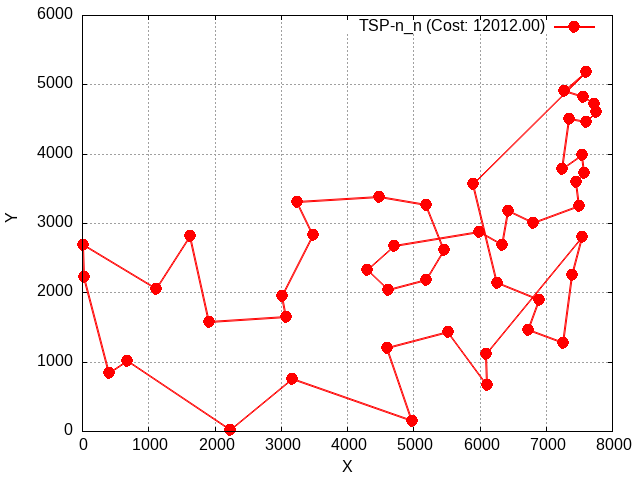
\includegraphics[width=0.7\textwidth]{images/TSP_n_n.png}
    \caption{Nearest Neighbor heuristic solution.}
    \label{fig:nn-example}
\end{figure}

Figure~\ref{fig:nn-example} illustrates the best tour obtained by running the Nearest Neighbor heuristic from each possible starting node on the \textit{Att48} instance. Several edge crossings are visible, indicating inefficiencies. The resulting tour cost is \textbf{12012}, significantly higher than the optimal cost of \textbf{10628}.

To address these limitations, the next section introduces the 2-opt heuristic, a simple yet effective local search technique aimed at improving tour quality by eliminating such inefficiencies.

\section{Two-Opt}

The \textit{2-opt} algorithm is a local search optimization technique designed to improve a given (possibly sub-optimal) tour 
in the Travelling Salesman Problem. It works by iteratively removing two edges from the tour and reconnecting the resulting paths 
in the opposite way, with the goal of reducing the overall cost of the cycle.
Formally, we can interpret 2-opt as a particular case of a more general class of heuristics known as \textit{k-opt}, 
where $k$ edges are removed and reconnected to form a new valid tour. In the 2-opt case, we identify two edges $(p_i, p_{i+1})$ 
and $(p_j, p_{j+1})$ such that replacing them with $(p_i, p_j)$ and $(p_{i+1}, p_{j+1})$, while reversing the intermediate segment between $p_{i+1}$ and $p_j$. 
The necessary condition for this move to be beneficial is:

The 2-opt move is beneficial only if replacing the two selected edges reduces the overall tour cost. 
Consider the current edges \((p_i, p_{i+1})\) and \((p_j, p_{j+1})\). 
We propose replacing them with \((p_i, p_j)\) and \((p_{i+1}, p_{j+1})\), 
which effectively reverses the intermediate segment of the tour.

The move is accepted if the total cost decreases, i.e., if:

\begin{equation}
    c(p_i, p_{i+1}) + c(p_j, p_{j+1}) > c(p_i, p_j) + c(p_{i+1}, p_{j+1})
    \label{eq:2opt-condition}
\end{equation}

Equivalently, the cost change \(\Delta\) resulting from this move can be computed as:

\begin{equation}
    \Delta = [c(p_i, p_j) + c(p_{i+1}, p_{j+1})] - [c(p_i, p_{i+1}) + c(p_j, p_{j+1})]
    \label{eq:2opt-delta}
\end{equation}

If \(\Delta < 0\), the move yields a shorter tour and is therefore accepted.

After identifying such a pair of edges, the segment of the tour between nodes $p_{i+1}$ and $p_j$ is reversed to maintain tour feasibility.

\begin{figure}[H]
    \centering
    \begin{subfigure}[c]{.4\textwidth}
        \centering
        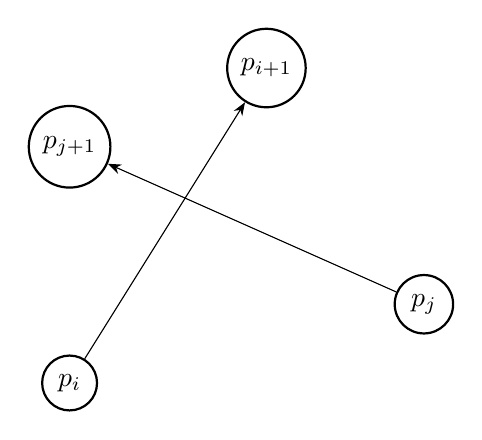
\begin{tikzpicture}
            \begin{scope}[every node/.style={circle,thick,draw}]
                \node (I) at (0,0) {$p_i$};
                \node (JJ) at (0,3) {$p_{j+1}$};
                \node (II) at (2.5,4) {$p_{i+1}$};
                \node (J) at (4.5,1) {$p_j$};
            \end{scope}
            \begin{scope}[>={Stealth[black]}, every node/.style={fill=white,circle},
                          every edge/.style={draw=red,very thick}]
                \draw[->,black] (I) -- (II);
                \draw[->,black] (J) -- (JJ);
            \end{scope}
        \end{tikzpicture}
        \caption{Before the move}
    \end{subfigure}
    \hfill
    \begin{subfigure}[c]{.4\textwidth}
        \centering
        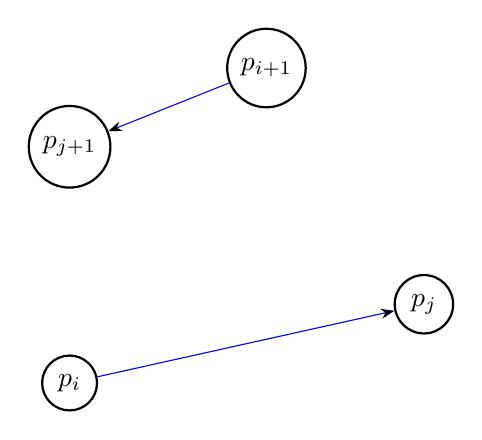
\begin{tikzpicture}
            \begin{scope}[every node/.style={circle,thick,draw}]
                \node (I) at (0,0) {$p_i$};
                \node (JJ) at (0,3) {$p_{j+1}$};
                \node (II) at (2.5,4) {$p_{i+1}$};
                \node (J) at (4.5,1) {$p_j$};
            \end{scope}
            \begin{scope}[>={Stealth[black]}, every node/.style={fill=white,circle},
                          every edge/.style={draw=blue,very thick}]
                \draw[->,blue] (I) -- (J);
                \draw[->,blue] (II) -- (JJ);
            \end{scope}
        \end{tikzpicture}
        \caption{After the move}
    \end{subfigure}
    \caption{Example of a 2-opt move eliminating edge crossing.}
    \label{fig:2optmove}
\end{figure}


As shown in Figure~\ref{fig:2optmove}, this operation is particularly useful in Euclidean instances, where removing intersecting edges 
usually improves the tour cost significantly. The process is repeated iteratively: at each step, the algorithm scans the tour looking 
for a pair of edges satisfying the inequality. If found, the edges are swapped and the search continues. 
When no further improvement can be found, the procedure terminates. This yields a solution that is often significantly better than the initial one, 
although not necessarily optimal.

To improve the Nearest Neighbor result, the 2-opt heuristic is applied as a post-processing step to the best tour found among all possible NN starting nodes. This selective refinement avoids unnecessary computation while still producing a significantly improved solution.

\subsection{Pseudocode}

\begin{algorithm}
\caption{Two-Opt Heuristic for TSP}
\label{alg:twoopt}
\textbf{Input:} A Hamiltonian cycle \texttt{solution} of a graph $G$, with associated cost\\
\textbf{Output:} An improved Hamiltonian cycle (locally optimal w.r.t. 2-opt), updated cost
\begin{algorithmic}
\Procedure{ApplyTwoOpt}{$solution$, $nnodes$}
    \State $improved \gets$ \textbf{true}
    \While{$improved$}
        \State $improved \gets$ \textbf{false}
        \For{$i \gets 0$ \textbf{to} $nnodes - 2$}
            \For{$j \gets i + 1$ \textbf{to} $nnodes - 1$}
                \State $\Delta \gets$ \Call{CostDelta}{$i$, $j$, $solution$}
                \If{$\Delta < 0$}
                    \State \Call{ReverseSubsequence}{$solution$, $i + 1$, $j$}
                    \State $solution.cost \gets solution.cost + \Delta$
                    \State $improved \gets$ \textbf{true}
                \EndIf
            \EndFor
        \EndFor
    \EndWhile
    \State \Return $solution$
\EndProcedure
\end{algorithmic}
\end{algorithm}

\begin{algorithm}
\caption{CostDelta and Subsequence Reversal}
\label{alg:subroutines}
\begin{algorithmic}
\Function{CostDelta}{$i$, $j$, $solution$}
    \State Let $p_i, p_{i+1}, p_j, p_{j+1}$ be the involved nodes
    \State \Return $c(p_i, p_j) + c(p_{i+1}, p_{j+1}) - c(p_i, p_{i+1}) - c(p_j, p_{j+1})$
\EndFunction

\Procedure{ReverseSubsequence}{$solution$, $start$, $end$}
    \State Reverse the order of nodes in $solution$ between indices $start$ and $end$ (inclusive)
\EndProcedure
\end{algorithmic}
\end{algorithm}

The \texttt{ApplyTwoOpt} procedure iteratively applies improving 2-opt moves until no further improvement is possible. 
The cost difference \texttt{CostDelta} evaluates the gain of removing two edges and reconnecting them in the opposite direction. 
If an improvement is found, the affected segment of the tour is reversed.

\subsection{Results Analysis}
To prove the effectiveness of the 2-opt approach, we apply it to the best tour generated by NN heuristic presented in Section \ref{sec:nn-analysis}.
Figure \ref{fig:nn-2opt-example} shows how this technique is as simple as it is effective. All edge crossings have been eliminated, resulting in a visibly more efficient tour.

\begin{figure}[h!]
    \centering
    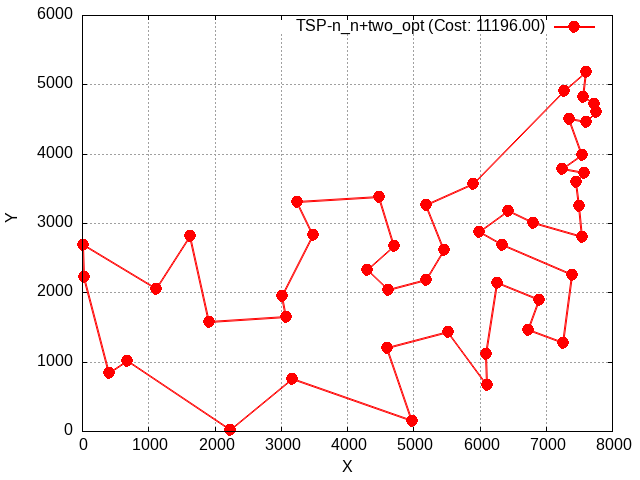
\includegraphics[width=0.7\textwidth]{images/TSP_n_n+two_opt.png}
    \caption{2-opt solution applied to the best tour generated by NN.}
    \label{fig:nn-2opt-example}
\end{figure}

To evaluate the improvement quantitatively, we can compare the cost of the tour before and after applying 2-opt and the computing time required to run both approaches. Table \ref{tab:nn-vs-2opt} summarizes the results of this comparison and highlights the significant reduction in tour cost achieved by the 2-opt heuristic, as well as the minimal increase in computation time.

\begin{table}[h!]
    \centering
    \caption{Comparison of tour cost and computation time.}
    \begin{tabular}{|c|c|c|}
        \hline
        Strategy & Cost & Time \\
        \hline
        NN        & 12012 & 0.006172 s \\
        \textbf{NN + 2opt} & \textbf{11196} & \textbf{0.006461 s} \\
        \hline
    \end{tabular}
    \label{tab:nn-vs-2opt}
\end{table}

These results are only meant to give an idea of the effectiveness of the 2-opt heuristic, some more rigorous analysis will be presented in Section XX \todo[inline]{Aggiungere riferimento alla sezione analisi perfprof}

\chapter{Metaheuristic}
\section{Metaheuristics}

A metaheuristic is a high-level, abstract problem-solving strategy designed to efficiently explore and exploit large solution spaces 
in complex optimization problems. Unlike algorithms tailored to specific instances, metaheuristics are general-purpose frameworks 
that guide subordinate heuristics—leveraging iterative improvement, intelligent search patterns, and adaptive behavior to find near-optimal solutions.

In our experiments, we employ metaheuristics that use the \textit{2-opt} algorithm as a foundational local search heuristic. 
Specifically, we take greedy solutions refined by 2-opt as initial configurations and further enhance them using one of two metaheuristic methods: 
\textbf{Tabu Search} and \textbf{Variable Neighborhood Search (VNS)}.

These strategies offer the ability to explore a broader search space than simple heuristics by incorporating mechanisms that allow 
occasional acceptance of worse solutions— thereby escaping local optima. We demonstrate that even relatively simple metaheuristic ideas, 
when combined with previously introduced heuristics, can yield solutions remarkably close to the optimal ones.

\section{Tabu Search}

Tabu Search is a metaheuristic developed to efficiently explore the solution space while avoiding local optima. 
Originally introduced by Fred Glover in 1986 and later formalized in 1989~\cite{Glover:TabuSearch}, it is well-suited for combinatorial problems like the Traveling Salesman Problem (TSP).

The method enhances a basic local search (in our case, 2-opt) by allowing non-improving moves and using a \textit{tabu list} to prevent cycling back to recently visited solutions.

\subsection{Search Strategy}

The search alternates between two phases:
\begin{itemize}
    \item \textbf{Intensification:} The algorithm performs 2-opt moves to locally improve the current solution.
    \item \textbf{Diversification:} When no improvement occurs for a specified number of iterations, a random move is introduced to escape local minima, 
        and the tabu tenure is increased to promote exploration.
\end{itemize}

\subsection{Implemented Mechanism}

In our implementation, the algorithm follows these steps:

\begin{enumerate}
    \item Generate an initial solution, either randomly or greedily.
    \item At each iteration, evaluate all possible 2-opt moves and select the best one not present in the tabu list.
    \item If the selected move does not improve the current solution, it is added to the tabu list.
    \item If a better solution is found and the tenure is greater than the minimum, the tenure is decreased to focus the search locally.
    \item If no improvement is made over a certain number of iterations, a random move is performed and the tenure is increased to enhance diversification.
\end{enumerate}

This results in a dynamic adjustment of the tabu tenure, based on the recent progress of the search, without relying on predefined functions or schedules.

\subsection{Tabu List Details}

Each tabu move corresponds to a 2-opt edge swap, and is represented by storing the two removed edges, $(p_i, p_{i+1})$ and $(p_j, p_{j+1})$. 
These moves are kept in the tabu list for a number of iterations defined by the current tenure. The list helps prevent the reversal of recent transformations 
and encourages the algorithm to explore new regions of the solution space.

\subsection{Pseudocode}

\begin{algorithm}
\caption{Tabu Search (simplified)}
\begin{algorithmic}
    \State $\text{sol} \gets$ initial solution
    \State $\text{best\_sol} \gets \text{sol}$
    \State $\text{tabulist} \gets \emptyset$
    \While{time limit not exceeded}
        \State $\text{move} \gets$ best 2-opt move not in tabu list
        \State Apply $\text{move}$ to $\text{sol}$
        \If{$\text{sol}$ is better than $\text{best\_sol}$}
            \State $\text{best\_sol} \gets \text{sol}$
            \If{tenure $>$ minimum}
                \State Decrease tenure
            \EndIf
        \Else
            \State Add $\text{move}$ to tabu list
            \State Increase counter for non-improving iterations
        \EndIf
        \If{counter exceeds threshold}
            \State Apply a random move
            \If{tenure $<$ maximum}
                \State Increase tenure
            \EndIf
        \EndIf
    \EndWhile
\end{algorithmic}
\end{algorithm}

The version of Tabu Search implemented here uses a simple yet adaptive strategy to balance exploration and exploitation. 
The dynamic adjustment of the tabu tenure—based on the quality of recent iterations—provides effective guidance through the solution space 
without introducing unnecessary complexity.

\clearpage

\section{Variable Neighborhood Search (VNS)}

A known limitation of the Tabu Search algorithm is the need to carefully tune several hyperparameters, such as the size and policy 
of the tabu list (static or dynamic tenure), which may be unaffordable in real-world scenarios and can lead to overfitting. 
Furthermore, diversification steps in Tabu Search might waste computational resources without significantly improving solution quality.

A simpler alternative is the \textit{Variable Neighborhood Search (VNS)} metaheuristic~\cite{Hansen2009}, 
which addresses the same problem from a different perspective. Rather than maintaining a tabu list to prevent reversals, 
VNS uses random \textit{k-opt} swaps, called \textbf{kicks}, to escape local minima. Since a k-opt move alters more than two edges, 
it is less likely to be undone by a simple 2-opt move.

\subsection{Algorithm Description}

The VNS algorithm iteratively improves a solution using 2-opt until no better neighbor is found. Then, it performs a series of random 3-opt kicks 
to perturb the solution and continues the search. This avoids complete restarts (as in multistart heuristics) and ensures better locality preservation.

The number of kicks is randomly selected within a fixed range $[k_{\text{min}}, k_{\text{max}}]$, making these the only hyperparameters of the method. 
Setting $k$ too high leads to excessive perturbation (mimicking a restart), while too few kicks may not help escape the local minimum. 
This trade-off is analyzed experimentally in Section~\ref{sec:results}. !!!!!!!!!!!!!!!TODO!!!!!!!!!!!!!!!!!!!

\begin{algorithm}
\caption{VNS}
\label{alg:vns}
\begin{algorithmic}
\Procedure{VNS}{$solution$}
    \State $solution \gets$ \Call{Greedy}{$solution$}
    \While{not \Call{Timeout}{}}
        \State $move \gets$ \Call{FindBest2OptSwap}{$solution$}
        \If{\Call{Delta}{$move$} $\leq 0$}
            \For{$i = 1$ to \Call{Random}{$k_{\min}, k_{\max}$}}
                \State $move \gets$ \Call{Random3OptSwap}{$solution$}
                \State $solution \gets$ \Call{Apply}{$solution$, $move$}
            \EndFor
        \Else
            \State $solution \gets$ \Call{Apply}{$solution$, $move$}
        \EndIf
    \EndWhile
    \State \Return $solution$
\EndProcedure
\end{algorithmic}
\end{algorithm}

\subsection{3-Opt Kick Structure}

Each kick is implemented as a 3-opt move affecting three edges. Figure~\ref{fig:3optkick} illustrates the transformation: 
three existing edges are removed, and three new ones are inserted, generating a different tour configuration. These kicks are stochastic and 
designed to avoid short cycles or reversals.

\begin{figure}[h]
    \centering
    \begin{subfigure}[c]{.4\textwidth}
        \centering
        \resizebox{\linewidth}{!}{
            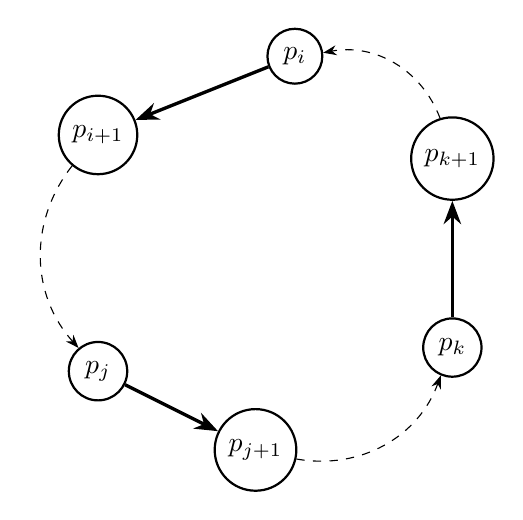
\begin{tikzpicture}
                \begin{scope}[every node/.style={circle,thick,draw}]
                    \node (I) at (2.5,4) {$p_i$};
                    \node (II) at (0,3) {$p_{i+1}$};
                    \node (J) at (0,0) {$p_j$};
                    \node (JJ) at (2,-1) {$p_{j+1}$};
                    \node (K) at (4.5,0.3) {$p_k$};
                    \node (KK) at (4.5,2.7) {$p_{k+1}$};
                \end{scope}

                \begin{scope}[>={Stealth[black]}, every node/.style={fill=white,circle},
                            every edge/.style={draw=red,very thick}]
                    \path[->] (I) edge[draw=black] (II);
                    \path[->] (J) edge[draw=black] (JJ);
                    \path[->] (K) edge[draw=black] (KK);
                    \path[->] (II) edge[dashed, draw=black, thin, bend right=40] (J);
                    \path[->] (JJ) edge[dashed, draw=black, thin, bend right=40] (K);
                    \path[->] (KK) edge[dashed, draw=black, thin, bend right=40] (I);
                \end{scope}
            \end{tikzpicture}
        }
    \end{subfigure}
    \hspace{1em}
    \raisebox{-0.5\height}{$\Rightarrow$}
    \hspace{1em}
    \begin{subfigure}[c]{.4\textwidth}
        \centering
        \resizebox{\linewidth}{!}{
            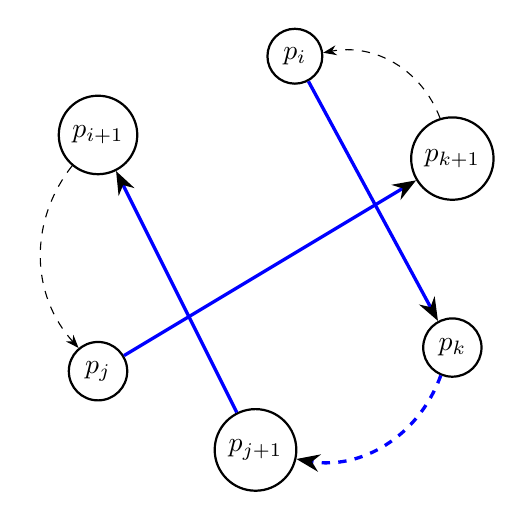
\begin{tikzpicture}
                \begin{scope}[every node/.style={circle,thick,draw}]
                    \node (I) at (2.5,4) {$p_i$};
                    \node (II) at (0,3) {$p_{i+1}$};
                    \node (J) at (0,0) {$p_j$};
                    \node (JJ) at (2,-1) {$p_{j+1}$};
                    \node (K) at (4.5,0.3) {$p_k$};
                    \node (KK) at (4.5,2.7) {$p_{k+1}$};
                \end{scope}

                \begin{scope}[>={Stealth[black]}, every node/.style={fill=white,circle},
                            every edge/.style={draw=red,very thick}]
                    \path[->] (I) edge[draw=blue] (K);
                    \path[->] (JJ) edge[draw=blue] (II);
                    \path[->] (J) edge[draw=blue] (KK);
                    \path[->] (II) edge[dashed, draw=black, thin, bend right=40] (J);
                    \path[->] (K) edge[dashed, draw=blue, bend left=40] (JJ);
                    \path[->] (KK) edge[dashed, draw=black, thin, bend right=40] (I);
                \end{scope}
            \end{tikzpicture}
        }
    \end{subfigure}
    \caption{Effect of a 3-opt kick applied to a TSP tour.}
    \label{fig:3optkick}
\end{figure}

In some cases, a single 3-opt is sufficient to escape a local minimum; in others, multiple perturbations are necessary. 
To handle this, we adopted a multithreaded strategy that performs parallel VNS searches with different numbers of kicks and selects 
the best result after reapplying 2-opt.

\subsection{Pseudocode}

\begin{algorithm}
\caption{VNS high-level pseudocode}
\label{alg:vns_highlevel}
\begin{algorithmic}
\State \textbf{Input:} starting node $s \in V$
\State \textbf{Output:} Hamiltonian cycle and its cost
\State
\State $(cycle, cost) \gets$ \Call{Greedy}{$s$, $V$}
\While{time not exceeded}
    \State $(cycle', cost') \gets$ \Call{ApplyRandom3OptKicks}{$cycle$}
    \State $(cycle', cost') \gets$ \Call{Apply2Opt}{$cycle'$}
    \If{$cost' < cost$}
        \State $(cycle, cost) \gets (cycle', cost')$
    \EndIf
\EndWhile
\State \Return $(cycle, cost)$
\end{algorithmic}
\end{algorithm}

\subsection{Performance and Comparison}

%The VNS algorithm consistently outperforms Tabu Search, yielding up to 3\% better results on average. 
%This improvement is primarily due to VNS’s lower dependence on fine-tuning and simpler logic, enabling better scalability and robustness.

\chapter{Exact Methods}
\label{chap:exact-methods}
Despite the promising results achievable with a well-designed heuristic, it is necessary to consider strategies aimed at finding the optimal solutions.

Before going into the implementation of exact methods, we must first examine the problem formulation introduced in Section~\ref{sec:prob-form}, particularly the Subtour Elimination Constraints (SECs) in Equation~\ref{eq:ilp_sec}. It is important to highlight that the number of SECs grows exponentially with respect to the number of nodes in the instance, making it infeasible to generate all of them upfront, even for problems of moderate size.

This section presents the implementation of exact methods whose goal is to generate SECs in a more intelligent and efficient manner, leveraging CPLEX to solve the resulting mathematical model.

\section{CPLEX}

CPLEX is a high-performance solver for linear programming (LP), mixed-integer programming (MIP), and quadratic programming problems. It is widely used in both academic research and industrial applications due to its efficiency, scalability, and support for advanced solving techniques. \cite{cplex2023}

It provides a rich set of APIs, allowing for integration into custom optimization workflows, along with powerful features like presolving, cutting planes, heuristics, and branch-and-bound algorithms. One of the most useful functionalities of CPLEX for combinatorial optimization problems, such as the Traveling Salesman Problem, is the support for \emph{callbacks}. These allow users to interact with the solver during the optimization process, for example, by adding constraints dynamically (lazy constraints) or customizing branching decisions.

In this work, CPLEX is used to solve the integer linear programming (ILP) formulation of the TSP, taking advantage of its support for dynamic constraint generation to efficiently handle the exponential number of Subtour Elimination Constraints.

\section{Benders Decomposition}

Benders Decomposition is a general technique for solving large-scale mixed-integer problems by iteratively decomposing them into a master problem and one or more subproblems. 

In our implementation, the main idea is to:
\begin{itemize}
    \item Solve a relaxed version of the ILP model without SECs.
    \item Analyze the resulting solution to detect subtours (disconnected components).
    \item Add one or more SECs to eliminate these subtours.
    \item Repeat the process until a connected solution is found.
\end{itemize}

\begin{figure}[H]
    \centering
    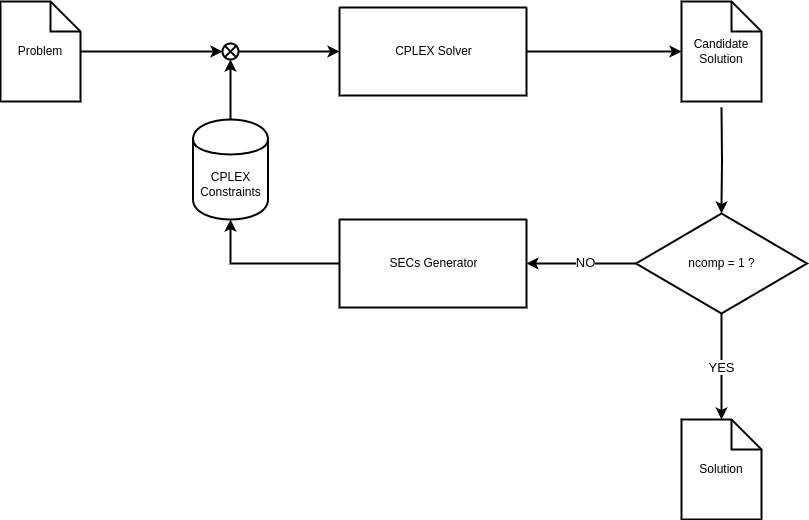
\includegraphics[width=0.9\textwidth]{benders_flow.drawio.png}
    \caption{Flowchart of the Benders-like solving loop for the TSP.}
    \label{fig:benders_flowchart}
\end{figure}

\subsection{Cycle Detection and SEC Addition.}
The solution provided by CPLEX after each iteration is typically fractional or disconnected. To restore feasibility, we apply a component detection procedure: all edges \( x_{ij} \) such that \( x_{ij} > 0.5 \) are considered part of the current solution, and a union-find-like structure is used to identify the connected components.

For each component \( C_k \), we add the following constraint:
\[
\sum_{\substack{i,j \in C_k \\ i \neq j}} x_{ij} \leq |C_k| - 1
\]
This ensures that in future iterations, such subtours will be avoided.

\subsection{Pseudocode}
\begin{algorithm}[H]
\caption{Subtour Elimination Loop}
\begin{algorithmic}[1]
\State Initialize \texttt{comp[i] = -1} for all nodes $i$, and set \texttt{ncomp = 0}
\Repeat
    \State Solve the relaxed ILP using \texttt{CPXmipopt}
    \State Extract solution and build components from $x^*_{ij} > 0.5$
    \State \texttt{ncomp} $\gets$ number of connected components
    \If{$ncomp > 1$}
        \For{each component $C_k$}
            \State Add SEC: $\sum_{i,j \in C_k} x_{ij} \leq |C_k| - 1$
        \EndFor
    \EndIf
\Until{\texttt{ncomp} = 1 or time limit reached}
\end{algorithmic}
\end{algorithm}

The entire loop is managed manually, CPLEX is invoked multiple times, at each iteration with an updated model that includes new constraints.

\subsection{Patching Heuristic}
\label{ssec:patching}
In cases where the solving loop exceeds the time limit or fails to converge to a single connected component, we introduce a fallback heuristic called \emph{patching}, which aims to merge disconnected subtours into a feasible Hamiltonian cycle.

The algorithm works as follows:
\begin{itemize}
    \item Identify all components (subtours) in the current solution.
    \item For each pair of components, consider removing an edge from one component and connecting its endpoint to a node in the other component.
    \item Compute the extra cost for each reconnection and select the pair that minimizes the increase in total cost.
    \item Repeat the operation until all components are merged into a single tour.
\end{itemize}

\begin{figure}[H]
    \centering
    \begin{subfigure}{0.45\textwidth}
        \centering
        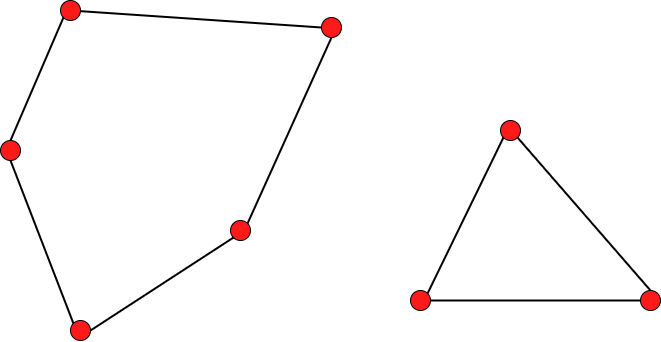
\includegraphics[width=\textwidth]{pre_patch.drawio.png}
        \caption{Disconnected subtours (MIP solution)}
        \label{fig:pre_patch}
    \end{subfigure}
    \hfill
    \begin{subfigure}{0.45\textwidth}
        \centering
        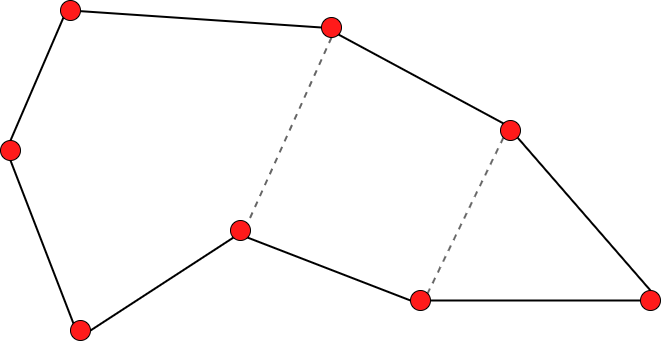
\includegraphics[width=\textwidth]{post_patch.drawio.png}
        \caption{Final tour after patching}
        \label{fig:post_patch}
    \end{subfigure}
    \caption{Visual example of the patching heuristic. The initial MIP solution contains multiple disconnected cycles (a), which are then merged into a single feasible tour (b) using edge reconnection.}
    \label{fig:patching_combined}
\end{figure}

Finally, once a patched tour is constructed, a local optimization phase (e.g., 2-opt) can optionally be applied to refine the solution quality. Obviously, this solution does not guarantee optimality, but it is a reliable fallback in case the Benders loop does not have enough time to reach the global minimum.

\section{Branch-and-Cut}

Branch-and-Cut is a state-of-the-art exact method for solving the TSP and many other combinatorial problems. It extends the classical Branch-and-Bound algorithm by dynamically adding valid inequalities (cuts) to the model, such as Subtour Elimination Constraints, during the exploration of the branch-and-bound tree.

In our implementation, we leverage CPLEX’s built-in support for lazy constraint callbacks to detect and eliminate subtours on-the-fly. This allows us to start from a relaxed ILP formulation and enforce connectivity only when needed, without pre-generating the exponential number of SECs.

\subsection{Lazy Constraint Mechanism}

Rather than rebuilding the model after each solution, Branch-and-Cut integrates subtour elimination directly into the solving loop through a callback mechanism. After each integer-feasible solution is identified by the solver, a callback is triggered to verify whether the current edge selection forms a valid Hamiltonian cycle. This is achieved by analyzing the connected components of the solution. If multiple subtours are found, one or more violated SECs are generated and dynamically injected into the model as lazy constraints.

This logic can be visualized using the flow in Figure~\ref{fig:benders_flowchart}, with the only difference being that SECs are injected directly into the CPLEX solver, and the model is not rebuilt from scratch at each iteration.

This interaction happens entirely within the solver, reducing overhead and fully exploiting CPLEX’s branch-and-bound engine. In our implementation, this is realized by registering a lazy constraint callback under the candidate solution context, which ensures that only integer-feasible solutions are inspected. The integration is fully transparent to the solver's internal mechanisms, preserving performance.

\subsection{Pseudocode}

\begin{algorithm}[H]
\caption{Callback-based Subtour Elimination}
\begin{algorithmic}[1]
\State Define lazy constraint callback function:
\Statex \quad Extract $x^*_{ij}$ from current solution
\Statex \quad Build connected components from $x^*_{ij} > 0.5$
\If{\texttt{ncomp} $>$ 1}
    \For{each component $C_k$}
        \State Add SEC: $\sum_{i,j \in C_k} x_{ij} \leq |C_k| - 1$
    \EndFor
\EndIf
\State Attach callback to CPLEX model
\State Solve the ILP using \texttt{CPXmipopt}
\end{algorithmic}
\end{algorithm}

The callback logic relies on identifying connected components from the edge variables $x_{ij}$ using a simple traversal procedure. Subtours are detected efficiently and corresponding SECs are added using CPLEX's lazy constraint API, avoiding the need to rebuild the model.

This structure ensures that any subtour detected during the search is immediately eliminated, allowing the solver to explore only feasible (or corrected) branches.


% Bibliography
%\clearpage{\pagestyle{plain}\cleardoublepage}
%\chapter{Bibliography}
%\input{chapters/bibliography}

\printbibliography

\end{document}
